%----------------------------------------------------------------------------------------
%	METODE
%----------------------------------------------------------------------------------------

\section*{METODE PENELITIAN}

Penelitian ini diawal dengan pengumpulan data selanjutnya masuk tahap ke indexing, kemudian membagi data tersebut menjadi data latih dan data uji. Data latih kemudian akan di klasifikasikan menggunakan metode klasifikasi Rocchio. Tahapan terakhir yaitu mengevaluasi hasil klasifikasi metode rochhio dengan data uji. Skema tahapan analisis sentimen dapat dilihat pada Gambar \ref{fig:tahapan} 

\begin{figure}[h!] % Gunakan \begin{figure*} untuk memasukkan Gambar
	\centering
	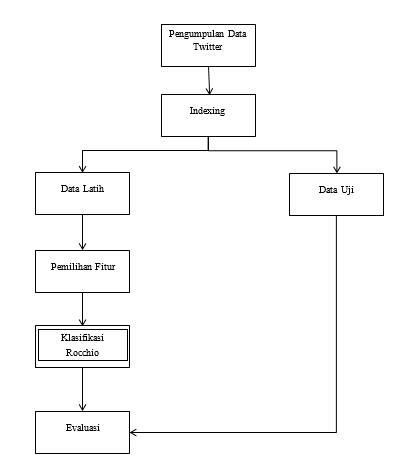
\includegraphics[width=200pt]{langkahkerja.png}
	\caption{Tahapan Penelitian Metode Klasifikasi Rocchio pada Sentimen Analisis Data Twitter}
	\label{fig:tahapan}
\end{figure}

\subsection*{Pengumpulan Data}
Tahapan dalam penelitian analisis sentimen ini yaitu diawali dengan pengumpulan data twitter. Data yang digunakan merupakan data \textit{post user}. \textit{Post} atau pesan dalam twitter dikenal dengan sebutan tweet (\cite{ZHANG2011}). Data yang akan diambil dari twitter adalah data dengan kata kunci “Kementrian” ,”mentri”, “Pendidikan”, “Sekolah”, dan “Indonesia”. Kata kunci tersebut digunakan  untuk mengambil data terkait opini – opini masyarakat di bidang kementrian dan pendidikan. Pada tahap akuisisi data tweet, data diperoleh dari tags.hawksey.info. Data yang didapatkan berupa data excel dengan atribut seperti yang terlihat pada Tabel \ref{tab:strukturdatatwitter}.

\begin{table}[hbt]
	\caption{Struktur Data Response Twitter}
	\centering
	\begin{tabular}{llr}
		
		\cmidrule(r){1-2}
		Atribut & Keterangan \\
		\midrule
		id\_str & id dari \textit{post} twitter \\
		from\_user & \textit{username} pemakai twitter \\
		text & \textit{post} twitter \\
		created\_at & tanggal dan waktu \textit{post} dibuat \\
		geo\_coordinates & koordinat tempat \textit{user} \\
		source & tautan profil \textit{user} \\
		profile\_image\_url & gambar profil dari \textit{user} \\
		user\_followers\_count & jumlah \textit{follower user} \\
		user\_friends\_count & jumlah teman \textit{user} \\
		user\_location & lokasi dari \textit{user} \\
		status\_url & link dari \textit{post} twitter \\
		
		\bottomrule
	\end{tabular}
	\label{tab:strukturdatatwitter}
\end{table}

Tabel \ref{tab:strukturdatatwitter} merupakan informasi struktur data Twitter yang diperoleh dari tags.hawksey.info. Data yang diperoleh dari sistem masih berupa data mentah post user yang belum ada sentimennya. Data dengan atribut text yang akan diambil untuk diproses selanjutnya. Data atribut text ini yang selanjutnya akan diolah sentimennya. Proses pengolahan data mentah menjadi sentimen dilakukan secara manual. Jumlah data yang digunakan pada penelitian ini sebanyak 6000 data yang sudah diberi sentimen. Dari data tersebut akan dibagi menjadi dua, yaitu data latih sebanyak 70\% dan data uji sebanyak 30\%. 


\subsection*{Indexing}

Setelah data didapatkan dan memiliki sentimen tahap selanjutnya yaitu \textit{indexing}. \textit{Indexing} merupakan proses persiapan yang dilakukan terhadap dokumen sehingga dokumen siap untuk diproses. Proses \textit{indexing} dibagi menjadi dua proses, yaitu \textit{document indexing} dan \textit{term indexing}. Dari \textit{term indexing} akan dihasilkan koleksi kata yang akan digunakan untuk meningkatkan performansi pencarian pada tahap selanjutnya. Selain itu, teknik \textit{indexing} ini juga dilakukan agar hasil yang diperoleh lebih baik. Karena kebanyakan \textit{tweet} hanya berisi tautan dan tidak menunjukkan sentimen tertentu, dan penulisannya ditulis dalam bahasa asing (Parikh dan Movassate 2014). Bahasa asing yang dimaksud dalam penelitian adalah kata – kata yang dalam penulisannya menggunakan pengabungan antara alfanumerik dan simbol – simbol lainnya. Ada beberapa tahapan  yang dilakukan didalam proses \textit{indexing} diantaranya \textit{tokenizing}, pengahapusan \textit{stopwords}, normalisasi kata, \textit{stemming}, dan pembuatan \textit{document term matrix}.


\subsubsection*{Tokenizing}
Tahap awal dalam proses \textit{indexing} adalah \textit{tokenizing}. Pada tahap ini setiap data \textit{post twitter} yang berupa kata – kata akan diubah menjadi kumpulan term, dengan tidak menyertakan mention, URL, tanda baca, dan angka pada \textit{tweet}. Selain itu, semua data pada tweet juga akan diubah menjadi huruf kecil. Proses memotong dokumen atau kata menjadi bagian-bagian yang lebih kecil disebut token. Token bisa berupa paragraf, kalimat, frasa kata tunggal sederhana, dan konsep. Teknik yang digunakan dalam proses tokenisasi adalah segmentasi dan memilah. Sebagai contoh, jika ada masukkan teks “Pendidikan Indonesia”, maka hasil keluaran dari proses \textit{tokenizing} adalah seperti yang disajikan pada Tabel \ref{tab:tokenizing}.

\begin{table}[hbt]
	\caption{Tokenizing}
	\centering
	\begin{tabular}{llr}
		\toprule
		Input & \multicolumn{2}{c}{Pendidikan Indonesia} \\
		\midrule
		Output & Pendidikan & Indonesia\\
		\bottomrule
	\end{tabular}
	\label{tab:tokenizing}
\end{table}

Tabel \ref{tab:tokenizing} merupakan contoh hasil proses \textit{tokenizing}, setiap kalimat yang ada akan dipilah menjadi potongan – potongan kata. Pada penelitian ini \textit{tokenizing} dilakukan dengan menggunakan kode dari Nette yang didapat dari https://github.com/nette/tokenizer.


\subsubsection*{Penghapusan Stopwords}

\textit{Stopwords} merupakan kata – kata atau term yang tidak berhubungan dan tidak memiliki makna atau informasi yang berhubungan dengan dokumen, walaupun kata tersebut sering muncul pada dokumen. \textit{Stopwords} adalah sebuah kata-kata dalam bahasa tertentu yang sangat umum digunakan dan memiliki nilai informasi nol (Meyer et.al . 2008). Penghapusan kata tersebut tidak akan mengubah makna dan isi dari informasi tweet, beberapa contoh stopwords dalam bahasa  Indonesia diantaranya: yang, juga, dari, dia, kami, kamu, aku, saya, ini, dan itu. Pada penelitian ini digunakan dataset daftar \textit{stopword} yang  didapatkan dari penelitian Tala (2003) sebanyak 759 kata. Dataset penelitian Tala inilah yang nantinya akan digunakan untuk menghapus \textit{stopword} pada data \textit{tweet}.


\subsubsection*{Normalisasi Kata}

Normalisasi kata merupakan proses penggantian kata yang tidak baku menjadi kata baku. Normalisasi ini dilakukan untuk mempermudah proses penelitian pada tahapan selanjutnya. Kata baku akan cenderung lebih kecil ambiguitas dibandingkan dengan kata yang tidak baku, untuk itu normalisasi dilakukan untuk mentranslasi kata tidak baku menjadi baku (Aziz 2013). Untuk itu perlu dilakukan normalisasi kata dengan cara mengganti kata yang tidak baku (Sproat et al. 2001). Pada penelitian ini proses pengantian kata tidak baku menjadi baku menggunakan dataset yang sudah ada. Dataset yang digunakan adalah sebuah kamus yang berisi kumpulan data tidak baku dengan kata bakunya. Hal ini dilakukan untuk memudahkan proses penggantian kata. Dataset kata tidak baku dan kata baku yang digunakan sebanyak 3719 baris data. 

\subsubsection*{Stemming}

\textit{Stemming} merupakan proses transformasi kata – kata menjadi kata dasarnya dalam sebuah teks dokumen, hal ini juga digunakan untuk meningkatkan performa IR (Agusta, 2009). \textit{Stemming} adalah  proses  konversi term ke  bentuk  umumnya. Tidak hanya ditransformasi menjadi kata dasar, tetapi kata – kata juga dapat ditransformasikan ke dalam bentuk sinonim kata tersebut. Sinonim adalah kata yang memiliki kesamaan makna tetapi berbeda dari sudut pandang morfologis. Contoh stemming dapat dilihat pada gambar \ref{fig:steming} 

\begin{figure}[h!] % Gunakan \begin{figure*} untuk memasukkan Gambar
	\centering
	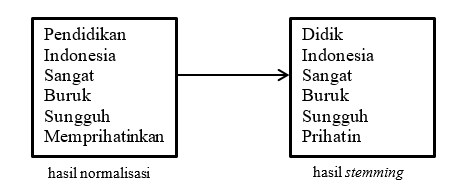
\includegraphics[width=200pt]{steming.png}
	\caption{Stemming}
	\label{fig:steming}
\end{figure}

Tahap \textit{stemming} bertujuan untuk mengurangi jumlah kata dan mendapatkan kata dasar yang benar-benar sesuai. Untuk itu penghapusan kata dan berbagai variasi lainnya seperti \textit{prefix} dan \textit{suffix} perlu dilakukan. Penelitian ini menggunakan algoritma Nazief dan Adriani (1996) dan kamus kata dasar  yang digunakan sebanyak 28.526 kata.

\subsubsection*{Pembuatan Document Term Matrix (DTM)}

\textit{Term Document Matrix} (TDM) dilakukan untuk menghitung jumlah kemunculan kata pada dokumen (Nadilah 2016). Cara yang paling umum untuk merepresentasikan teks ke dalam bentuk matrik adalah melalui pembuatan DTM. DTM dapat diekspor dari korpus dan digunakan sebagai mekanisme \textit{bag-of-words}. Pendekatan ini menghasilkan matrik dengan id dokumen sebagai baris dan \textit{term} sebagai kolom. Setiap elemen matrik yang ada merupakan representasi dari frekuensi kemunculan kata.
Sebagai contoh ada dua dokumen dengan id 1 dan 2 mempunyai kata yang sama yaitu “Saya suka makan nasi dan saya suka ayam goreng” dan “ayam goreng”. Tabel \ref{tab:dtm} menunjukkan contoh DTM yang terbentuk.
.

\begin{table}[hbt]
	\caption{Document Term Matrix}
	\centering
	\begin{adjustbox}{max width=\textwidth}
		\begin{tabular}{*{7}{c}}%%{llr}
			\toprule
			ID & saya & suka & makan & nasi & dan & ayam \\
			\midrule
			1 & 2 & 2 & 1 & 1 & 1 & 1 \\
			2 & 0 & 0 & 0 & 0 & 1 & 1 \\
			\bottomrule
		\end{tabular}
	\end{adjustbox}
	\label{tab:dtm}
\end{table}

Sedangkan pada penelitian ini, kolom matriks menunjukkan kata yang ada pada data \textit{tweet}, dan baris matriks menunjukkan indeks dari dokumen pada kumpulan korpus. Pada penelitian ini satu tweet menandakan satu dokumen.

\subsection*{Pembagian Data}

Data yang dihasilkan setelah proses \textit{indexing} dibagi  menjadi  dua subset data yaitu data latih dan data uji dengan perbandingan 70:30. Sebanyak 70 persen data latih dan 30 persen data uji. Data latih ini akan digunakan untuk tahapan selanjutnya sementara data uji digunakan untuk melakukan pengujian terhadap sistem klasifikasi yang telah dibuat dalam penelitian ini.

\subsection*{Pemilihan Fitur}

Pemilihan fitur merupakan proses pemilihan term yang mewakili informasi penting dari suatu dokumen atau teks. Adanya pemilihan fitur ini dapat meningkatkan akurasi karena adanya seleksi pada \textit{term} yang bukan merupakan penciri (Manning et all. 2008). Menurut Garnes (2009) pemilihan fitur secara umum dibagi menjadi dua metode, yaitu \textit{unsupervised feature selection} dan \textit{supervised feature selection}. Metode \textit{Unsupervised feature selection} tidak menggunakan informasi kelas dalam data latih ketika memilih fitur untuk \textit{classifier}, contohnya adalah \textit{Inverse Document Frequency} (IDF). 

Sedangkan \textit{Supervised feature selection}  adalah metode seleksi fitur yang menggunakan informasi kelas dalam data latih, sehingga \textit{set pre-classied} harus tersedia agar seleksi fitur dapat dilakukan. 

Pada penelitian ini pemilihan fitur yang akan digunaka yaitu IDF. IDF dipilih karena metode ini efisien, mudah dan memiliki hasil yang akurat (Robertson 2005).


\subsubsection*{Inverse document frequency (IDF)}

\textit{Inverse Document Frequency} (IDF) merupakan salah satu metode yang digunakan dalam pemilihan fiitur.  Sebelum masuk ke tahapan klasifikasi, pembobotan dilakukan pada setiap data yang ada untuk dapat menghitung kesamaan dan jarak antar data traning dengan data uji. Pada Penelitian ini untuk menghitung bobot setiap kata dalam dokumen digunakan skema pembobotan IDF.
 
\textit{Inverse document frequency} (IDF) adalah \textit{inverse} atau kebalikan dari nilai DF. Hal ini dikarenakan \textit{term} yang sering muncul di dokumen dianggap sebagai term umum, sehingga tidak penting nilainya, sehingga ukuran kepentingan suatu term dari dokumen yang akan digunakan penciri yang memiliki nilai kecil dengan rentang yang tidak begitu jauh. Sebaliknya \textit{term} yang jarang muncul pada dokumen perlu diperhatikan dalam pembobotan. Menurut Witten (1999) kata yang jarang atau paling sedikit muncul justru harus diperhatikan sebagai kata yang lebih penting dari pada kata yang paling sering muncul dalam dokumen. Banyaknya dokumen $d$ yang mengandung \textit{term} $t$ tertentu disebut DF. Ukuran kepentingan suatu \textit{term} dari dokumen yang digunakan sebagai penciri adalah nilai DF yang besar, namun nilai dari DF memiliki rentang nilai yang lebar. Nilai IDF dapat diperoleh  dengan formula
\begin{equation}
idf\textsubscript{t} = log(\frac{N}{df\textsubscript{t}})
\end{equation}
variabel N adalah banyaknya dokumen dan sedangkan df adalah banyaknya dokumen didalam koleksi yang mengandung \textit{term} tertentu, sehingga dapat dikatakan bahwa IDF merupakan frekuensi \textit{term} atau data yang jarang muncul dalam suatu dokumen.



\subsection*{Klasifikasi}
Pada analisis sentimen klasifikasi digunakan untuk mengkategorikan setiap data yang ada ke kelas pencirinya. Salah satu tujuan dari klasifikasi teks atau dokumen adalah penggolongkan atau mengelompokkan suatu dokumen ke dalam suatu kategori tertentu
(\cite{MANNING2008}). Klasifikasi juga bertujuan untuk memprediksi karakteristik dari suatu objek. Klasifikasi juga dapat digunakan untuk mendeteksi sentimen terhadap suatu isu. Data hasil indexing akan diklasifikasikan terhadap analisis sentiment. Pada penelitian ini terdiri 3 kelas sentimen yang digunakan, yaitu positif, negatif, dan netral. Fungsi klasifikasi secara umum untuk memetakan suatu dokumen ke dalam kategori tertentu yaitu
\begin{equation}
\begin{split}
\tiny
\gamma : X -> C
\label{eq:klasifikasi}
\normalsize
\end{split}
\end{equation}
secara umum fungsi ini yang akan dipakai untuk mengelompok data ke dalam himpunan kelas atau kategori yang ada, dengan X adalah kumpulan dokumen dan C merupakan kategori. Fungsi klasifikasi terbagi menjadi dua metode yaitu, berbasis vektor dan berbasis peluang (\cite{MANNING2008}). 

Secara garis besar pada pendekataan berbasis peluang, penentuan kelas pada sebuah dokumen atau data adalah dengan cara menghitung peluang keberadaan data tersebut dalam suatu kelas. Naïve Bayes merupakan contoh pendekatan berbasis peluang. Sedangkan pada pendekatan berbasis vektor, penentuan kelas pada sebuah data dilakukan dengan cara menghitung jarak data tersebut ke \textit{centroid} suatu kelas. Metode yang dapat digunakan pada pendekatan ini adalah metode \textit{Rocchio algorithm}, \textit{k-Nearest Neighbor}, \textit{Descision Tree}, dan \textit{Support Vector Machines}. 

\textit{Metode Naïve Bayes} menghitung probabilitas dari suatu dokumen untuk masuk ke suatu kategori berdasarkan pada kehadiran dari kata yang sama di dalam dokumen lain yang telah ada di dalam kategori tersebut. Kelemahan dari metode ini adalah akurasinya yang rendah dari pada model lainnya. Metode Rocchio membandingkan dokumen terhadap suatu daftar term positif dan negatif bagi setiap katagori dan mengklasifikasikan sesuai dengan kehadiran atau bobot dari term-term tersebut. Metode rocchio memiliki komputasi yang tidak rumit sederhana dan mudah, tetapi kelemahan dari metode ini adalah akurasi yang rendah (Bashiri et al, 2005). Pada \textit{kNearest Neighbor} klasifikasi ini mencari sebanyak k dokumen paling mirip dan menempatkan dokumen ke kategori di mana k dokumen tersebut ditempatkan sebelumnya, metode ini memiliki kinerja yang baik, terutama dengan penempatan banyak kategori, tetapi waktu klasifikasi relatif lama karena pada setiap proses klasifikasi harus menentukan k tetangga terdekat dan sangat sulit untuk mendapatkan nilai k yang optimal. Metode \textit{Decision Tree} memisahkan dokumen - dokumen secara hirarki di dalam struktur pohon, di mana setiap node merupakan term yang relevan dan ujung setiap cabang adalah kategori. Metode ini lebih mudah dipahami, mudah untuk menyusun aturan keputusan, dan dapat mengurangi kompleksitas komputasi, tetapi metode ini memiliki kelemahan yaitu jika pada penentuan root terdapat kesalahan maka hal ini akan menyebabkan kesalahan juga pada node level di bawahnya. Sedangkan pada \textit{Support Vector Machines}, metode menggambar antara term yang berkontribusi dan tidak terhadap suatu dokumen yang akan ditempatkan ke suatu kategori tertentu. Kategori didasarkan pada kehadiran dari term yang berkontribusi. Metode ini merupakan yang terbaik meskipun sangat mudah terjadi \textit{error} dalam data \textit{ training}.

\textit{Naïve bayes} dan \textit{Rocchio} sama-sama memiliki kelemahan dari segi akurasinya, dan kecepatan dalam segi komputasi yang relatif sama hanya saja kedua metode ini memiliki basis yang berbeda. \textit{Naïve bayes} berbasis peluang dan \textit{Rocchio} berbasis vektor. Untuk itu pada penelitian ini akan membandingkan kedua metode ini, manakah diantara kedua metode ini yang memiliki tingkat hasil akurasi lebih baik untuk klasifikasi.


\subsubsection*{Metode Naive Bayes}
Model klasifikasi Multinomial dan Bernoulli merupakan metode klasifikasi berbasis peluang yang paling sering digunakan. Model klasifikasi ini banyak digunakan karena mudah diaplikasikan dan prosesnya sederhana (\cite{MANNING2008}). Pada model Multinomial Bernoulli  setiap dokumen memiliki atribut yang menunjukkan ada atau tidaknya kata- kata atau \textit{term} dalam dokumen tersebut, tetapi jumlah kemunculan term dalam dokumen tidak ikut diperhitungkan. Pada model Multinomial \textit{Naïve Bayes}, jumlah kemunculan term pada dokumen ikut diperhitungkan, setiap dokumen diwakili oleh kemunculan \textit{term} dari dokumen. Pada model ini, dapat diasumsikan jika kemunculan masing-masing term t bersifat independen antara satu term dengan yang lainnya. Dengan menggunakan nilai dari $P(c|d)$ peluang suatu dokumen $d$ di dalam kelas $c$ dapat ditulis sebagai (\cite{MANNING2008}) 
\begin{equation}
\begin{split}
P(C|d) \alpha P(c) \Xi_{1\le k\le nd}P(t_k|c)
\label{eq:multinb}
\end{split}
\end{equation}
dengan $P(tk|c)$ adalah peluang dari suatu term $tk$ muncul pada dokumen $d$ yang diketahui memiliki kelas $c$. Pendugaan parameter $P (tk|c)$ dihitung dengan formula
\begin{equation}
\begin{split}
\tiny
P(t_k|C) = \frac{T_{ct}}{\sum _{t' \in V} T_{ct'}}
\label{eq:multinblanjut}
\normalsize
\end{split}
\end{equation}
dengan T$_\alpha$ adalah jumlah kemunculan term t dalam dokumen training yang berada di kelas $c$.  adalah jumlah seluruh term yang muncul berulang kali pada dokumen yang sama (\cite{MANNING2008}).

\textit{Term} tidak selalu muncul pada salah satu kelas saat dilakukan klasifikasi sehinggga nilai $P (tk|c)$ yang dihasilkan adalah nol. Untuk mengatasi permasalahan tersebut, digunakan laplace smoothing, yaitu menambahkan frekuensi term sebanyak 1 sehingga perhitungan dari $P(tk |c)$  menjadi 
\begin{equation}
\begin{split}
\tiny
P(t_k|C) = \frac{T_{ct}}{\sum _{t' \in V} T_{ct'} + B}
\label{eq:multinblanjutb}
\normalsize
\end{split}
\end{equation}

\subsubsection*{Metode Rocchio}
Klasifikasi ini merupakan salah satu metode pembelajaran \textit{supervised document classification}. Metode \textit{Rocchio relevance feedback} adalah strategi reformulasi query paling populer karena sering digunakan untuk membantu user pemula suatu \textit{information retrieval systems} (Joachims 2013). Dalam siklus \textit{relevance feedback}, kepada user disajikan hasil pencarian dokumen, setelah itu user dapat memeriksa dan menandai dokumen yang benar-benar relevan Klasifikasi yang digunakan pada penelitian ini adalah fungsi klasifikasi dengan basis vektor, yaitu metode klasifikasi Rocchio. Klasifikasi rocchio merepresentasikan data ke dalam sebuah vektor. Kedekatan kesamaan isi dihitung dari kedekatan sudut yang terbentuk antara bobot data training dan bobot data test menggunakan aturan sodinus. Untuk menghitung bobot setiap kata dalam dokumen digunakan skema pembobotan TFIDF (Term Frequency / Invers Document Frequency) karena komponen heuristic utama adalah dalam klasifikasi rocchio yaitu skema pembobtan tfidf, untuk itu metode pembelajaran rocchio disebut juga dengan TFIDF Classifiers (Joachihms 1997). Pendekatan ini menggunakan perhitungan jarak atau kemiripan suatu data dengan pusat sebuah kelas. Metode ini membagi ruang vektor menjadi beberapa bagian berdasarkan centroid yang ada. 

Pada penelitian ini setiap dokumen training direpresentasikan sebagai vektor. Setiap titik atau vektor dokumen traning akan diberikan label sesuai dengan kategori kelasnya. Contohnya saja seperti pada Gambar \ref{fig:rocio} 

\begin{figure}[h!] % Gunakan \begin{figure*} untuk memasukkan Gambar
	\centering
	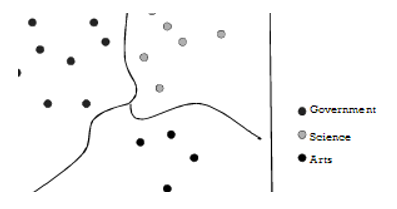
\includegraphics[width=200pt]{rocio.png}
	\caption{Pelabelan pada kategori kelas}
	\label{fig:rocio}
\end{figure}

Teknik Rocchio menerapkan batas - batas tersebut dalam bentuk\textit{ centroid} untuk memberi batasan tersebut. Nilai \textit{centroid} ini didapat dengan menghitung rata- rata jarak pada setiap data atau dokumen. \textit{Centroid} dapat diperoleh dengan
\begin{equation}
\begin{split}
\mu (c) = \frac{1}{D_{c}} \sum \limits_{d\in D_c} v(d)
\label{eq:rociosatu}
\end{split}
\end{equation}
selanjutnya dari masing masing vektor dokumen akan dicari nilai centroidnya dari setiap kelas yang ada menggunakan persamaan (10). Persamaan diatas digunakan untuk menghitung centroid dari kelas C, dimana Dc merupakan kumpulan dari dokumen di dalam korpus c, sedangkan v(d) merupakan vektor dokumen yang telah dinormalisasi. Terdapat dua cara untuk menentukan kemiripan dua vektor space model yaitu dengan mengukur jarak atau mengukur kemiripan. Untuk menentukan jarak kedekatan data uji ke dalam suatu kelas adalah dengan menghitung jarak antara kedua vektor menggunakan persamaan \textit{Euclidean}, yang didefinisikan sebagai berikut
\begin{equation}
\begin{split}
|d_1 - d_2 | = \sqrt{\sum_{i=1}^{m}(x_i - y_i)^2}
\label{eq:rociodua}
\end{split}
\end{equation}
sedangkan untuk menghitung kemiripan antara dua vektor dokumen, yaitu
\begin{equation}
\begin{split}
sim(d_1, d_2) = \frac{v(d_1).v(d_2)}{|v(d_1)||v(d_2)|}
\label{eq:rociotiga}
\end{split}
\end{equation}

Pada penelitian ini pendekatan yang akan digunakan untuk mencari kemiripan antara dua vector adalah pendekatan \textit{similarity}, sedangkan untuk pembobotannya digunakan IDF. Pendekatan ini digunakan karena pendekatan \textit{similarity} mencari kemiripan berdasarkan kesamaan, bukan berdasarkan kedekatan. Sedangkan pada pendekatan jarak, pengukuran dilakukan berdasarkan kedekatan. Kedekatan belum tentu menunjukkan kesamaan antar \textit{term}. Untuk itulah pendekatan menggunakan \textit{similarity} yang akan digunakan, yang selanjutnya diharapkan resiko kesalahan dalam pengambilan dokumen akan lebih sedikit terjadi.

\subsection*{Evaluasi}
Tahapan evaluasi adalah tahapan untuk mengetahui tingkat akurasi dan kinerja dari hasil klasifikasi menggunakan metode Rocchio. Kinerja klasifikasi dievaluasi dengan cara menghitung nilai akurasi, \textit{recall}, \textit{precision}, dan \textit{F-measure} dengan bantuan tabel \textit{confusion matrix}. \textit{Token} dari hasil seleksi fitur, akan dihitung peluangnya berdasarkan kelas-kelasnya dari dokumen Twitter. Setelah itu, membandingkannya dengan kelas aktual dari data uji dan kelas hasil prediksi dengan menggunakan \textit{confusion matrix}.
Menurut \citeauthor{MANNING2008} (\cite*{MANNING2008}) terdapat dua parameter yang umum digunakan untuk mengukur kinerja sebuah sistem temu kembali informasi, yaitu \textit{precision} dan \textit{recall} Pengukuran efektivitas dilakukan untuk mengevaluasi system IR. Perlu adanya suatu tolak ukur yang digunakan untuk mengukur kualitas hasil klasifikasi. Pengukuran selanjutnya akan mengunakan nilai precision, recall, akurasi, dan F1. 

\subsection*{Precision}
\textit{Precision} adalah jumlah kelompok dokumen relevan dari total jumlah dokumen yang  ditemukan oleh sistem. \textit{Precision} direpresentasikan sebagai presentase dokumen yang di-retrieve yang benar-benar relevan, seperti yang ditunjukkan pada persamaan
\begin{equation}
\begin{split}
Precision = \frac{\#(relevant items retrieved)}{\#(retrieved items)} \\ 
= P(relevant|retrieved)
\label{eq:precision}
\end{split}
\end{equation}

\subsection*{Recall}
\textit{Recall} adalah rasio jumlah dokumen relevan yang ditemukan kembali dengan total jumlah dokumen dalam kumpulan dokumen yang dianggap relevan. \textit{Recall} dapat dihitung dengan 
\begin{equation}
\begin{split}
Recall = \frac{\#(relevant items retrieved)}{\#(relevant items)} \\ 
= P(retrieved|relevant)
\label{eq:recall}
\end{split}
\end{equation}


\subsection*{Akurasi}
Setelah nilai precision dan recall didapatkan keakuratan hasil klasifikasi juga dinilai dari akurasinya, kemudian membandingkannya dengan kelas aktual dari data uji dan kelas hasil prediksi dengan menggunakan \textit{confusion matrix} untuk untuk menghitung akurasi digunakan rumus seperti berikut dan mengacu tabel \textit{confusion matrix} pada Table \ref{tab:konsep}. 

\begin{table}[hbt]
	\caption{Tabel Kontigensi}
	\centering
	\begin{adjustbox}{max width=\textwidth}
		\begin{tabular}{*{4}{c}}%%{llr}
			\toprule
			 & Positif & Netral & Negatif \\
			\midrule
			Positif & TP & FNt1 & FNg1 \\
			Netral & FP1 & TNt & FNg2 \\
			Negatif & FP2 & FNt2 & TNg \\
			\bottomrule
		\end{tabular}
	\end{adjustbox}
	\label{tab:konsep}
\end{table}

Penelitian ini membagi tiga sentimen yaitu positif , netral , dan negatif. Untuk itu table \textit{confusion matrix} akan memiliki kolom dan baris yang direpresentasikan seperti Tabel \ref{tab:konsep}. Pada Tabel \ref{tab:konsep} TP menunjukkan semua prediksi yang benar untuk data aktual positif, FP1 dan FP2 adalah jumlah prediksiyang salah untuk data aktual positif, TNt adalah jumlah prediksi yang benar untuk data aktual netral, FNt1 dan FNt2 adalah jumlah prediksi yang salah untuk data aktual netral, TNg menunjukkan jumlah prediksi yang benar untuk data aktual negatif, sedangkan FNg1 dan FNg1 menunjukkan jumlah prediksi yang salah untuk data aktual negatif. Dari Tabel \ref{tab:konsep} selanjutnya nilai akurasi dapat diperoleh dengan menggunakan formula
\begin{equation}
\begin{split}
\tiny
accuracy = (tp+tn)/(tp+fp+fn+tn)
\label{eq:akurasi}
\normalsize
\end{split}
\end{equation}
selanjutnya akan menghasilkan nilai akurasi hasil klasifikasi yang berupa pembagian dari penjumlahaan nilai benar actual positif, negatif , dan netral dengan semua penjumlahan nilai prediksi yang didapat.

\subsection*{F-measure}
Pengukuran selanjutnya adalah dengan menggunakan F-measure yang merupakan \textit{weighted harmonic mean} dari \textit{precision} dan \textit{recall}.Dimana $\alpha$ $\in$ [0,1] dan $\beta^2$ $\in$ [0, $\Psi$] dengan
\begin{equation}
\begin{split}
F = \frac{1}{\alpha \frac{1}{p} + (1 - \alpha)\frac{1}{R}} \\
= \frac{(\beta^2 + 1)PR}{\beta^2P + R} \\
where \beta^2 = \frac{1 - \alpha}{\alpha}
\label{eq:fmeasure}
\end{split}
\end{equation}


Balanced F-measure menyamakan bobot dari precision dan recall, yang berarti membuat $\alpha$ = 1/2 atau $\beta$ = 1. Ketika menggunakan $\beta$ = 1, persamaan \ref{eq:fmeasure} dapat disederhanakan  menjadi persamaan
\begin{equation}
\begin{split}
\tiny
F_\beta = \frac{2PR}{P + R}
\label{eq:fmeasuredua}
\normalsize
\end{split}
\end{equation}
dimana P adalah \textit{precision}, dan R adalah \textit{recall}.

\subsection*{Jadwal Kegiatan}
Penelitian ini akan dilakukan selama 4.5 bulan dengan rincian kegiatan seperti tercantum pada Tabel \ref{tab:jadwal}.
\begin{table*}[t!]
	\begin{center}
		\caption{Rencana Jadwal Penelitian}
		\label{tab:jadwal}
		\footnotesize
		\begin{tabular}{|l|c|c|c|c|c|c|c|c|c|c|c|c|c|c|c|c|c|c|}
			\hline
			\multirow{2}{*}{Kegiatan}&\multicolumn{2}{c|}{1}&\multicolumn{4}{c|}{2}&\multicolumn{4}{c|}{3}&\multicolumn{4}{c|}{4}&\multicolumn{4}{c|}{5}\\
			\cline{2-19}
			&3&4&1&2&3&4&1&2&3&4&1&2&3&4&1&2&3&4\\
			\hline
			Penyusunan Proposal Skripsi&\cellcolor{black}&\cellcolor{black}&\cellcolor{black}&\cellcolor{black}&&&&&&&&&&&&&&\\
			\hline
			Kolokium&&&&&\cellcolor{black}&&&&&&&&&&&&&\\
			\hline
			Perbaikan proposal&&&&&&\cellcolor{black}&&&&&&&&&&&&\\
			\hline
			Pengambilan data Twitter&&&&&&\cellcolor{black}&\cellcolor{black}&\cellcolor{black}&&&&&&&&&&\\
			\hline
			Pembuatan sistem analisis sentimen &&&&&&&&\cellcolor{black}&\cellcolor{black}&\cellcolor{black}&\cellcolor{black}&&&&&&&\\
			\hline
			Penulisan draft skripsi&&&&&&&&&&&&\cellcolor{black}&\cellcolor{black}&\cellcolor{black}&\cellcolor{black}&&&\\
			\hline
			Uji sistem&&&&&&&&&&&&&&&&\cellcolor{black}&&\\
			\hline
			Sidang skripsi&&&&&&&&&&&&&&&&&\cellcolor{black}&\\
			\hline
			Perbaikan laporan penelitian&&&&&&&&&&&&&&&&&&\cellcolor{black}\\
			\hline
		\end{tabular}
		\normalsize
	\end{center}
\end{table*}